\chapter{基于团树传播的精确推断}
\label{chap:pgm-junction-tree}

设备报警后，诊断程序先询问故障概率，随后又要计算过热概率，以及故障与传感器失灵的联合概率。对这几个查询分别运行第~\ref{chap:pgm-elimination}章的变量消除，会多次完成相同的局部求和。把这些中间表连同其依赖的因子和证据保存下来，后续查询就能接着计算。

这种按依赖关系保存的中间因子称为\term{消息}（message）。消息以边界变量的取值为输入，记录边界一侧的因子在消去内部变量后的结果。树的一条边把计算分成两侧，因而可以直接确定消息汇总的范围。对于含环的图，本章先把需要共同处理的变量组成团，再把团连成保留全部共享变量的树，随后用双向消息支持多次查询和局部证据更新。

以下以有限离散变量为对象，使用取有限非负值的因子。变量索引组成集合$V$，$X_i$的状态集合记为$\mathcal{X}_i$；$\bm{x}_A$表示索引集合$A\subseteq V$上一组变量取值。推断过程中模型参数固定，每个求和都遍历所标变量的全部状态，空乘积取$1$。

\section{从变量消除到消息传递}
\label{sec:pgm-junction-tree-from-elimination}

继续考虑设备诊断：二元变量$F,H,A,S$依次表示故障、过热、报警和传感器失灵，联合分布分解为
\begin{equation}
  p(f,h,a,s)=p(f)p(h\mid f)p(s)p(a\mid h,s).
  \label{eq:pgm-junction-tree-device}
\end{equation}
取$p(F=1)=0.1$、$p(S=1)=0.05$，以及$p(H=1\mid F=0)=0.1$、$p(H=1\mid F=1)=0.8$。表~\ref{tab:pgm-junction-tree-alarm-cpt}给出各状态下的报警概率；对应的未报警概率由$1$减去该值获得。这组人工设置的参数用于展示计算过程。

\begin{table}[htbp]
  \centering
  \begin{tabular}{ccc}
    \toprule
    $h$ & $s$ & $p(A=1\mid h,s)$\\
    \midrule
    $0$ & $0$ & $0.01$\\
    $1$ & $0$ & $0.90$\\
    $0$ & $1$ & $0.70$\\
    $1$ & $1$ & $0.99$\\
    \bottomrule
  \end{tabular}
  \caption{设备诊断例的报警条件概率。传感器正常时，过热使报警概率由$0.01$升至$0.90$；传感器失灵时，即使没有过热，报警概率也达到$0.70$。}
  \label{tab:pgm-junction-tree-alarm-cpt}
\end{table}

给定报警证据$A=1$，查询故障概率时先对传感器状态求和，形成关于$H$的表
\begin{equation}
  u(h)=\sum_s p(s)p(A=1\mid h,s),
  \qquad (u(0),u(1))=(0.0445,0.9045).
  \label{eq:pgm-junction-tree-boundary-likelihood}
\end{equation}
表$u(h)$已把传感器状态汇总完毕。保持模型参数和报警证据不变，故障查询和过热查询都可以读取这张表；它记录的是给定过热状态时报警侧的贡献。从另一侧消去故障变量，则得到
\begin{equation}
  v(h)=\sum_f p(f)p(h\mid f),
  \qquad (v(0),v(1))=(0.83,0.17).
  \label{eq:pgm-junction-tree-boundary-prior}
\end{equation}
表$v(h)$仅由故障先验和过热条件概率形成，可以在报警证据变化后继续使用。两侧通过同一个$h$组合，得到$p(h,A=1)=u(h)v(h)$。再对$h$归一化或求和，就能回答不同查询。

消息传递把中间表的变量、来源和更新方向一并记录。图~\ref{fig:pgm-junction-tree-factor-cut}给出本例的树状因子图：切断$H$与报警因子的连接后，两侧只共享$H$。给定$h$，左侧对故障求和得到$v(h)$，右侧对报警和传感器状态求和得到$u(h)$。保存整个关于$h$的函数表，使后续计算可以按所需边界状态读取；单次变量消除也可以采用这种缓存方式。

\begin{figure}[htbp]
  \centering
  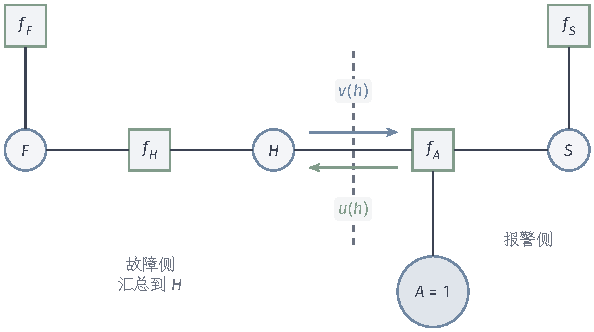
\includegraphics[width=100.651mm]{figures/06-probabilistic-graphical-models/02-inference/tikz/pgm-junction-tree-factor-cut/figure.pdf}
  \caption{设备诊断例的树状因子图。圆节点是变量，方框是因子，证据$A=1$附在报警变量处。虚线所切的两侧以$H$为共同边界，蓝色消息$v(h)$汇总故障侧，绿色消息$u(h)$汇总报警侧；箭头指示消息的发送方向。}
  \label{fig:pgm-junction-tree-factor-cut}
\end{figure}

按边界状态保存子问题结果，是动态规划在这里的具体形式。树边两侧的内部变量互不重叠，各侧的结果可以直接组合。含环图上的消息可能沿不同路径再次带回同一因子的贡献，因此需要另行处理重叠的依赖范围。

\section{树结构上的消息传递}
\label{sec:pgm-junction-tree-tree-messages}

在因子图中，因子$f_\alpha$对作用域$D_\alpha\subseteq V$中的变量进行局部计算，全部因子的索引组成$\mathcal{F}$。每个变量至少连接一个因子；孤立变量可接入恒为$1$的一元因子，以便用统一的消息形式处理。变量$i$处的证据记为$\ell_i(x_i)$：未观测时取$1$，观测$X_i=e_i$时取$\mathbf{1}\{x_i=e_i\}$。全部证据$\bm e$对应的权重和条件分布为
\begin{equation}
  \begin{aligned}
    q_{\bm{e}}(\bm{x})
      &=\prod_{\alpha\in\mathcal{F}}f_\alpha(\bm{x}_{D_\alpha})
        \prod_{i\in V}\ell_i(x_i),\\
    Z_{\bm{e}}&=\sum_{\bm{x}}q_{\bm{e}}(\bm{x}),\qquad
    p(\bm{x}\mid\bm{e})=\frac{q_{\bm{e}}(\bm{x})}{Z_{\bm{e}}}.
  \end{aligned}
  \label{eq:pgm-junction-tree-evidence-weight}
\end{equation}
当$Z_{\bm e}>0$时，归一化得到条件分布。观测变量仍留在图中，其后验质量集中在观测值上，因此证据变化时可以继续使用同一组变量和连接。对于无证据配分函数为$Z_0$的未归一化模型，硬证据概率等于$Z_{\bm e}/Z_0$；只有$Z_0=1$时才直接等于$Z_{\bm e}$。

\subsection{和积消息}
\label{sec:pgm-junction-tree-sum-product}

先设因子图连通且无环。变量$i$的相邻因子集合为$N(i)$，因子$\alpha$的相邻变量集合为$N(\alpha)=D_\alpha$。\term{和积消息}（sum-product message）将各分支的权重相乘，再对内部变量求和，留下接收方需要的变量。两类节点的更新式分别是
\begin{equation}
  m_{i\to\alpha}(x_i)
    =\ell_i(x_i)
      \prod_{\beta\in N(i)\setminus\{\alpha\}}
      m_{\beta\to i}(x_i),
  \label{eq:pgm-junction-tree-variable-message}
\end{equation}
\begin{equation}
  m_{\alpha\to i}(x_i)
    =\sum_{\bm{x}_{D_\alpha\setminus\{i\}}}
      f_\alpha(\bm{x}_{D_\alpha})
      \prod_{j\in D_\alpha\setminus\{i\}}
      m_{j\to\alpha}(x_j).
  \label{eq:pgm-junction-tree-factor-message}
\end{equation}
变量节点处的证据和入站消息都依赖同一个$x_i$，逐项相乘即可得到发出的表。因子节点则先固定接收变量$x_i$，把因子与其余变量的入站消息相乘，再遍历这些变量的状态求和。两类消息的输出都以$x_i$为索引。

乘积中排除接收方，是为了让消息只汇总发送侧。切断边$(i,\alpha)$，来自$\alpha$的消息汇总另一侧，乘入它就会重复计数。因子发送消息时，删除$\alpha$使其余邻接变量分属互不重叠的分支；给定这些变量的状态，各分支先独立求和。将结果与$f_\alpha$相乘，再消去接收变量以外的变量，便得到式~\eqref{eq:pgm-junction-tree-factor-message}。

把本例的四个因子写成$f_F=p(f)$、$f_H=p(h\mid f)$、$f_S=p(s)$、$f_A=p(a\mid h,s)$。从叶端开始，故障和传感器变量分别发送$m_{F\to f_H}(f)=p(f)$、$m_{S\to f_A}(s)=p(s)$；报警变量发送证据表$m_{A\to f_A}(a)=\mathbf{1}\{a=1\}$。两个相邻因子随后向$H$发送
\[
  \begin{aligned}
    m_{f_H\to H}(h)&=\sum_f p(h\mid f)p(f)=v(h),\\
    m_{f_A\to H}(h)&=\sum_{a,s}p(a\mid h,s)
       \mathbf{1}\{a=1\}p(s)=u(h).
  \end{aligned}
\]
$H$处没有额外证据，因此发往报警因子的消息为$m_{H\to f_A}=v$，发往故障因子的消息为$m_{H\to f_H}=u$。同一条边的两个方向分别携带两侧的汇总结果，各自具有不同的因子来源。树上的许多动态规划都可写成这样的局部和积运算\scite{pgm-overview-kschischang2001}

\subsection{消息调度与边缘恢复}
\label{sec:pgm-junction-tree-scheduling}

每次发送前，节点先等待除接收方之外的全部入站消息。选一个变量节点为根，从叶端向根进行\term{收集}（collect）：叶变量发送$\ell_i$，叶因子发送自身的一元函数，其余节点在分支结果到齐后继续向上发送。根收到各侧贡献后，再向叶端进行\term{分发}（distribute），使每个节点都能收到来自父侧的贡献。

有$M$条边的因子树共计算$2M$条有向消息，每条边的两个方向各一次。收集按叶到根的依赖顺序完成，分发再按根到叶的顺序完成，这两轮计算就能结束。根的边缘只需收集结果；查询其他位置的边缘时，分发提供它们所缺的另一侧信息。

把全部入站消息与节点处的局部输入组合，得到
\begin{equation}
  \begin{aligned}
    B_i(x_i)&=\ell_i(x_i)\prod_{\alpha\in N(i)}
       m_{\alpha\to i}(x_i),\\
    B_\alpha(\bm{x}_{D_\alpha})
      &=f_\alpha(\bm{x}_{D_\alpha})
        \prod_{j\in D_\alpha}m_{j\to\alpha}(x_j).
  \end{aligned}
  \label{eq:pgm-junction-tree-factor-beliefs}
\end{equation}
围绕$i$或$\alpha$切开树，各分支汇总其余因子，因而$B_i=\sum_{\bm{x}_{V\setminus\{i\}}}q_{\bm e}$、$B_\alpha=\sum_{\bm{x}_{V\setminus D_\alpha}}q_{\bm e}$。除以$Z_{\bm e}$，两者就是相应的后验边缘。若$i,j\in D_\alpha$，还可对$B_\alpha$的其余变量求和，得到$p(x_i,x_j\mid\bm e)$。成对因子的作用域正好覆盖原变量交互图的一条边；在二部因子图中，这两个变量通过同一个因子节点相连。

报警例的$H$处给出
\begin{equation}
  (B_H(0),B_H(1))=(0.036935,0.153765),
  \qquad Z_{\bm{e}}=0.19070.
  \label{eq:pgm-junction-tree-alarm-normalizer}
\end{equation}
据此得到$p(H=1\mid A=1)\approx0.806319$。向故障侧分发时，先计算$m_{f_H\to F}(f)=\sum_h p(h\mid f)u(h)=(0.1305,0.7325)$，再乘故障先验。故障状态$F=1$的权重为$0.07325$，归一化得到$p(F=1\mid A=1)=0.07325/0.19070\approx0.384111$。

这些数值保留了消息的原始尺度。为降低连乘下溢的风险，可以将非零消息整体除以正数；最终将局部汇总表归一化，后验边缘保持不变。此时$B_i$的总和带有消息缩放后的尺度，计算证据概率还需要保存并恢复缩放常数。全零消息表示发送侧在所有边界状态下都没有与证据相容的正权重配置，应保留这项零权重信息。

\subsection{最大积消息}
\label{sec:pgm-junction-tree-max-product}

寻找完整状态的最优解释时，要比较各配置的权重，而非累加它们。\term{最大积消息}（max-product message）以边界状态为索引，保存一侧子树能取得的最大权重。用$\nu$表示这套消息，将和积公式中的求和换成最大化，得到
\begin{equation}
  \begin{aligned}
    \nu_{i\to\alpha}(x_i)
      &=\ell_i(x_i)\prod_{\beta\in N(i)\setminus\{\alpha\}}
         \nu_{\beta\to i}(x_i),\\
    \nu_{\alpha\to i}(x_i)
      &=\max_{\bm{x}_{D_\alpha\setminus\{i\}}}
         f_\alpha(\bm{x}_{D_\alpha})
         \prod_{j\in D_\alpha\setminus\{i\}}
         \nu_{j\to\alpha}(x_j).
  \end{aligned}
  \label{eq:pgm-junction-tree-factor-max}
\end{equation}
由于分支变量互不重叠且因子非负，$\max_{\bm y,\bm z}g(\bm y)h(\bm z)=(\max_{\bm y}g)(\max_{\bm z}h)$，各侧最优值可以相乘。为了恢复最优配置，计算$\nu_{\alpha\to i}(x_i)$时，同时保存一组达到最大值的$\bm{x}_{D_\alpha\setminus\{i\}}$。这张从边界状态查找内部最优选择的表称为\term{回溯记录}（backpointer）。

将最大积入站消息全部组合，形成$\widehat{B}_i(x_i)=\ell_i(x_i)\prod_{\alpha\in N(i)}\nu_{\alpha\to i}(x_i)$。它记录固定$x_i$时全图的最大权重，称为\term{最大边缘}（max-marginal）。同一边界状态下，最大边缘取一组最优配置的权重，概率边缘则累加全部配置的权重。

收集后先在根处选择使证据与入站消息乘积最大的状态，再逐层读取回溯表：父变量状态确定后，查出相邻因子其余变量的状态，继续进入各分支。出现平局时，按固定顺序记录其中一组选择，回溯保持这组条件选择的关联。例如两个二元变量仅在$(0,0)$和$(1,1)$上权重为$1$，其余权重为零；两处最大边缘都对$0,1$平局，独立选择可能得到零权重的$(0,1)$。沿回溯记录选择，才能取得一组相容的最优解。

在设备诊断例中，以$H$为根，故障侧发送的最大权重为
\[
  \begin{aligned}
    \nu_{f_H\to H}(0)&=\max(0.9\times0.9,\;0.1\times0.2)=0.81,\\
    \nu_{f_H\to H}(1)&=\max(0.9\times0.1,\;0.1\times0.8)=0.09.
  \end{aligned}
\]
这两个$h$状态的回溯表都选$f=0$。报警侧在$h=0$时比较$0.95\times0.01$和$0.05\times0.70$，选$s=1$，权重为$0.035$；在$h=1$时比较$0.95\times0.90$和$0.05\times0.99$，选$s=0$，权重为$0.855$。根处的两个候选值为$0.02835$和$0.07695$，分别来自$0.81\times0.035$和$0.09\times0.855$，因此选$h=1$。回溯得到MPE配置$(f,h,s)=(0,1,0)$，未归一化权重为$0.07695$；报警变量保持证据值$A=1$。式~\eqref{eq:pgm-junction-tree-boundary-prior}和式~\eqref{eq:pgm-junction-tree-boundary-likelihood}中的和积表汇总全部配置，需与这套最大积表分别保存。

对于隐状态链，记状态为$Z_t$、观测为$X_t=x_t$。最大积收集依次向时间后端汇总，写成
\[
  \delta_t(z_t)=p(x_t\mid z_t)
    \max_{z_{t-1}}\{\delta_{t-1}(z_{t-1})p(z_t\mid z_{t-1})\}.
\]
从$\delta_1(z_1)=p(z_1)p(x_1\mid z_1)$开始，为每个$z_t$保存最优前驱状态，再由末端向前回溯，就得到Viterbi动态规划。它求解全部隐状态的联合最优配置，第~\ref{sec:pgm-dynamic-discrete}节将用于离散时序模型。若查询仅最大化部分变量，其余变量仍须求和，应采用第~\ref{sec:pgm-elimination-map}节的边缘MAP顺序。

\section{团树的构造}
\label{sec:pgm-junction-tree-construction}

含环因子图的两侧可能共享多个变量。将这些变量共同保留在消息中，便可以把一片局部计算组合成新的节点。\term{团树}（junction tree）的节点就是这样的变量团，边上的分隔集记录相邻团共享的变量。一个变量可能出现在多个团中，树上连接这些团的整条路径都须保留它，才能按同一个状态组合各处的因子。

图~\ref{fig:pgm-junction-tree-triangulation}以四环说明构造过程。消元产生的共同作用域先由填充边记录，随后用极大团容纳这些变量。将极大团连接起来，以交集为消息边界，再为原始因子选择存放位置，即可沿树边汇总两侧贡献。填充边和团节点用于组织计算，原联合分布仍由原始因子的乘积给出。

\begin{figure*}[htbp]
  \centering
  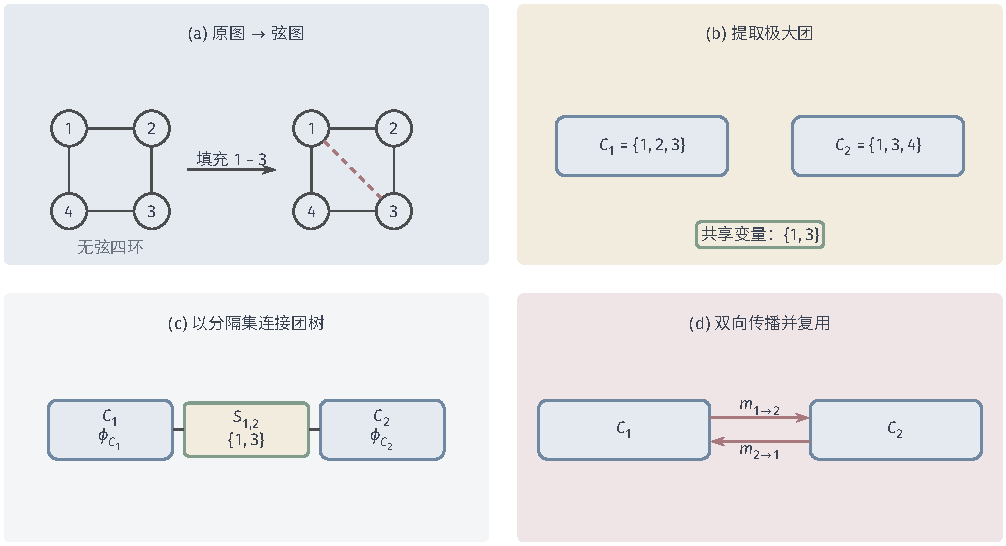
\includegraphics[width=169.000mm]{figures/06-probabilistic-graphical-models/02-inference/tikz/pgm-junction-tree-triangulation/figure.pdf}
  \caption{四环模型的团树构造与传播。添加填充边$1-3$后，两个极大团为$C_1=\{1,2,3\}$、$C_2=\{1,3,4\}$，共享变量组成分隔集$S_{1,2}=\{1,3\}$。最后一个面板在团间保存双向消息，用分隔集的状态组合两侧计算结果。}
  \label{fig:pgm-junction-tree-triangulation}
\end{figure*}

\subsection{从原图到弦图}
\label{sec:pgm-junction-tree-chordalization}

每个原始因子的全部变量需要放在同一个团内。有向模型的因子$p(x_i\mid\bm{x}_{\operatorname{pa}(i)})$涉及$i$及其父节点，因此先把共同子节点的父节点相连，再去掉方向，形成承载全部因子的道德图。这里保留全部变量，而条件独立检验会按具体查询选取祖先子图。在报警例中，两个报警父节点$H,S$由此相连，形成团$\{F,H\}$和$\{H,A,S\}$。

无向模型直接使用承载因子作用域的变量图；因子图则先将每个作用域中的变量两两相连。选定消元顺序后，每次把当前节点的剩余邻居全部相连，再移去该节点。将新增边保留在原变量集合上，得到\term{三角化}（triangulation）或弦化后的图；其中长度至少为$4$的环都有弦。

第~\ref{sec:pgm-elimination-complexity}节的最小度和最小填充启发式分别按剩余邻居数和缺失邻居边数选节点。填充记录消元后新因子的共同变量，每一步的求和仍完整保留被消变量的贡献。合法顺序给出相同的概率答案，但中间表和后续消息的规模可能不同。

完成填充后，所选顺序中每个节点的剩余邻居都两两相连，所以该顺序是完美消元序，所得图为弦图（参见\BookTheoremRef{thm:graph-theory-chordal-perfect-elimination}{卷1《数学准备：计算、分析与几何》第9章“图的表示与计算”第9.3.2.3节“弦图条件下的无填充分解”}）。

填充保留消元需要的共同作用域，数值计算继续使用原因子和原参数。

对四环$1-2-3-4-1$，先消去$2$会添加$1-3$，形成极大团$\{1,2,3\}$、$\{1,3,4\}$；先消去$1$则添加$2-4$，形成$\{1,2,4\}$、$\{2,3,4\}$，如图~\ref{fig:pgm-junction-tree-triangulation}所示。两种计算都保留原分布，消息的索引却分别为$\{1,3\}$和$\{2,4\}$。这两个变量组的状态数决定了不同的消息表成本。

\subsection{极大团、分隔集与运行交集性质}
\label{sec:pgm-junction-tree-running-intersection}

团中的变量两两相连。\term{极大团}（maximal clique）指已无法加入其他节点的团；它可以小于全图节点数最多的团。记全部极大团为$\mathcal C$，以它们为节点构造树$\mathcal T=(\mathcal C,\mathcal E_{\mathcal T})$。相邻团$C,D$的交集$S_{C,D}=C\cap D$称为\term{分隔集}（separator），消息以其中变量的共同取值为索引。

图~\ref{fig:pgm-junction-tree-running-intersection}上排把$\{1,2\}$、$\{2,3\}$、$\{3,4\}$依次连接。含$2$的两团相邻，含$3$的两团也相邻，$1,4$各只出现在一团中。下排把$\{3,4\}$移到中间，连接含$2$的两团时就需要经过一个不含$2$的团，消息无法在这条路径上保留$x_2$。

共享变量需要沿整条团间路径传递。若路径中途删去$i$，另一端的因子仍需与发送端按同一个$x_i$组合，而传到那里时已经没有这个索引。因此对团的连接还要施加以下条件。

\begin{definition}[运行交集性质]
  \label{def:pgm-junction-tree-running-intersection}
  团树满足\term{运行交集性质}（running intersection property），是指对任意变量$i$，包含$i$的全部团构成连通子树。等价地，对任意两个团$C,D$，从$C$到$D$的唯一路径上的每个团都包含$C\cap D$。
\end{definition}

树中任意两团之间只有一条路径。包含$i$的团若构成连通子树，这条路径上的团都含$i$；反过来，若任意两处之间的路径都保留$i$，含$i$的团就相互连通。

\begin{figure}[htbp]
  \centering
  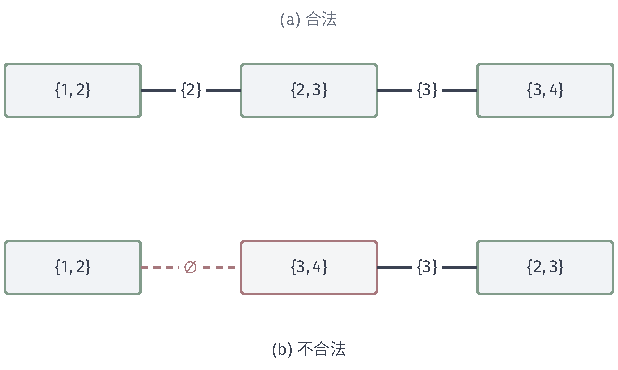
\includegraphics[width=104.652mm]{figures/06-probabilistic-graphical-models/02-inference/tikz/pgm-junction-tree-running-intersection/figure.pdf}
  \caption{运行交集性质的两种连接示例。上排每个变量出现的团都连续相连；下排连接含$2$的两团时，中间团$\{3,4\}$缺少$2$，沿该路径计算的消息会丢失共同状态$x_2$。}
  \label{fig:pgm-junction-tree-running-intersection}
\end{figure}

运行交集确定了每条消息需要保留的完整边界。删除边$(C,D)$，记$C$侧的团集合为$\mathcal C_{C\mid D}$，其中所有变量的并集为$U_{C\mid D}=\bigcup_{K\in\mathcal C_{C\mid D}}K$，则两侧的共同变量满足
\begin{equation}
  U_{C\mid D}\cap U_{D\mid C}=S_{C,D}.
  \label{eq:pgm-junction-tree-cut-intersection}
\end{equation}
$S_{C,D}$中的变量属于边的两端，所以一定出现在两侧。反之，若$i$在两侧的某个团中各出现一次，连接这两个团的路径经过$(C,D)$，运行交集迫使$C,D$都含$i$。因此两侧交集恰为$S_{C,D}$，消息可以消去其余内部变量。

给定分隔集状态，两侧便可各自求和，再相乘，这正是团树动态规划的分解方式。分配律和完整的边界保证结果精确；稠密离散表的成本仍指数依赖所选顺序的诱导宽度。实际计算需要团的状态空间足够小，能够存储并遍历这些表。

遗漏共享变量会改变求和结果。为二元链的三个团依次分配$\mathbf{1}\{x_1=x_2\}$、$\mathbf{1}\{x_2=x_3\}$、$\mathbf{1}\{x_3=x_4\}$，全局仅全$0$和全$1$的配置有非零权重，权重总和为$2$。若使用下排的错误连接，并以$\{1,2\}$为根，$\{2,3\}$先向$\{3,4\}$发送常数$1$，后者再经空分隔集向根发送标量$2$。根的求和得到$2\times2=4$：本应共享的$x_2$被分别消去，使两个局部求和组合了彼此不相容的状态。

\subsection{团树构造与因子分配}
\label{sec:pgm-junction-tree-spanning-tree}

弦图的极大团可以通过\term{团交图}（clique intersection graph）选择连接：以极大团为节点，将两团的交集大小
\[
  w(C,D)=|C\cap D|
\]
用作边权。非空交集产生正权边；对于不连通的原图，可用零权边连接不同分量，此时消息只携带空分隔集上的标量。以下把零权边也加入候选，以统一处理各连通分量。

对于非空有限弦图，把全部极大团作为节点，以交集大小为边权构成完全团图，其中保留交集为空的零权边。满足运行交集的生成树，恰好是总交集权最大的生成树（参见\BookTheoremRef{thm:graph-theory-clique-tree-maximum-weight}{卷1《数学准备：计算、分析与几何》第9章“图的表示与计算”第9.3.2.3节“弦图条件下的无填充分解”}）。选好团间连接后，还要为团分配概率因子，计算消息和边缘。

可以用最大权Kruskal算法选边。将候选边按权重从大到小排列，平局按固定顺序处理；从空边集开始，只有两端尚未连通时才加入当前边，以保持无环。选出$|\mathcal C|-1$条边、使全部团连通后，即得到所需的最大权生成树。

对于图~\ref{fig:pgm-junction-tree-running-intersection}中的三个团，$\{1,2\}$与$\{2,3\}$共享$2$，$\{2,3\}$与$\{3,4\}$共享$3$，首尾两团交集为空。候选边权为$1,1,0$，先加入的两条正权边已经形成上排的链。余下的零权边连接已连通的两端，会形成环，因此跳过。

定理适用于已完成三角化的弦图。四环的四个边团就无法组成运行交集树，选最大权生成树也会丢失某个共享变量。三角化先决定极大团的规模，最大权选边随后保证同一变量所在的团连续相连；这一步并不优化先前的消元顺序。图模型教材进一步讨论了分解图、团树与局部计算的关系\scite{pgm-lauritzen1996}

确定树以后，将每个原始因子$f_\alpha$存入一个覆盖其全部变量的团$a(\alpha)$，即$D_\alpha\subseteq a(\alpha)$。每个因子恰好分配一次，从而得到无证据团势
\begin{equation}
  \phi_C^0(\bm{x}_C)
    =\prod_{\alpha:\,a(\alpha)=C}f_\alpha(\bm{x}_{D_\alpha}),
  \qquad
  \prod_{C\in\mathcal{C}}\phi_C^0
    =\prod_{\alpha\in\mathcal{F}}f_\alpha.
  \label{eq:pgm-junction-tree-factor-assignment}
\end{equation}
未分到因子的团取势$1$。一个因子即使被多个团覆盖，也只存放一份，否则重复乘入会改变原乘积。报警例中取$C_1=\{F,H\}$、$C_2=\{H,A,S\}$，分别存放$\phi_{C_1}^0=p(f)p(h\mid f)$、$\phi_{C_2}^0=p(s)p(a\mid h,s)$，两团通过$H$组合。

合法的分配位置、最大权树和三角化可能有多种选择，它们都保留原始因子乘积，却形成不同的局部表和缓存依赖。选择时需同时考虑消息复用和表格规模：即使团树只有很少节点，一个大团也可能需要难以容纳的状态表。

\section{团树传播}
\label{sec:pgm-junction-tree-propagation}

运行交集已经确定两团之间的完整边界。下面沿这些边界进行数值计算，将因子树上的单变量消息推广为多变量表。本节分别保存每条边的双向消息，每次从局部输入和其他入站消息重新形成输出；公式只含乘法与求和，可以保留因子和证据中的零表项。

\subsection{团势与团间消息}
\label{sec:pgm-junction-tree-clique-messages}

\term{团势}（clique potential）保存分配给该团的原始因子及证据，取值非负，通常尚未归一化。它是局部计算的输入，传播完成后的边缘还需汇合全树的消息。为变量证据$\ell_i$选择一个含$i$的团$h(i)$，定义
\begin{equation}
  \phi_C(\bm{x}_C)=\phi_C^0(\bm{x}_C)
    \prod_{i:\,h(i)=C}\ell_i(x_i).
  \label{eq:pgm-junction-tree-local-evidence}
\end{equation}
每个原始因子和证据都恰好出现一次，因此$\prod_C\phi_C=q_{\bm e}$。多变量观测似然也可按相同方式吸收，但需由一个团覆盖全部作用域，并给出该似然的观测含义。一般软证据重复分配会重复乘入其权重，改变目标分布。

记团$C$的邻居集合为$N_{\mathcal T}(C)$。图~\ref{fig:pgm-junction-tree-message}展示发送$C\to D$的步骤：将$\phi_C$与除$D$之外的入站消息相乘，再对$C\setminus S_{C,D}$求和，留下分隔集上的表。反向消息按同一公式汇总$D$侧；两条消息一起提供共享变量两侧的完整贡献。

\begin{figure*}[htbp]
  \centering
  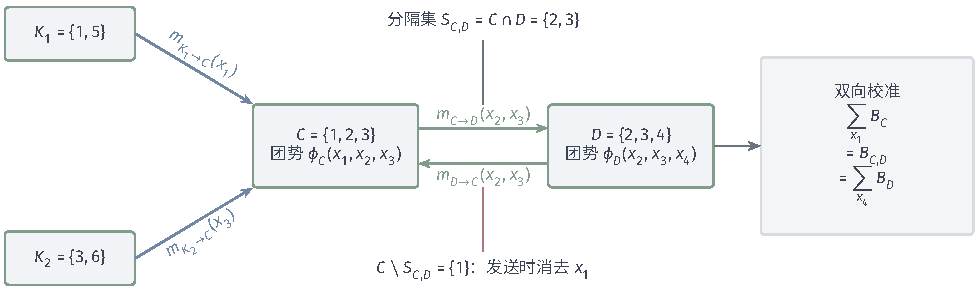
\includegraphics[width=165.650mm]{figures/06-probabilistic-graphical-models/02-inference/tikz/pgm-junction-tree-message/figure.pdf}
  \caption{团间消息与共享变量的汇总。蓝色入站消息与$\phi_C$相乘后，消去$C\setminus S_{C,D}=\{1\}$，得到以$\{2,3\}$为索引的$m_{C\to D}$；$D$侧消息留待后续组合。右侧两个方向的绿色消息共同形成$B_{C,D}$，校准后相邻团分别消去非共享变量，也得到这张分隔集表。}
  \label{fig:pgm-junction-tree-message}
\end{figure*}

对应的消息公式为
\begin{equation}
  m_{C\to D}(\bm{x}_{S_{C,D}})
    =\sum_{\bm{x}_{C\setminus S_{C,D}}}
      \phi_C(\bm{x}_C)
      \prod_{K\in N_{\mathcal{T}}(C)\setminus\{D\}}
        m_{K\to C}(\bm{x}_{S_{K,C}}).
  \label{eq:pgm-junction-tree-clique-message}
\end{equation}
计算乘积时，各函数按共同变量的状态对齐，较小作用域的函数在其余坐标上重复取值。局部势$\phi_C$保留原来的输入；新的消息另行保存，供其他方向的发送和后续查询使用。

将局部势与全部入站消息组合，并将一条边的两个方向消息组合，分别定义
\begin{equation}
  \begin{aligned}
    B_C(\bm{x}_C)
      &=\phi_C(\bm{x}_C)
        \prod_{K\in N_{\mathcal{T}}(C)}
          m_{K\to C}(\bm{x}_{S_{K,C}}),\\
    B_{C,D}(\bm{x}_{S_{C,D}})
      &=m_{C\to D}(\bm{x}_{S_{C,D}})
        m_{D\to C}(\bm{x}_{S_{C,D}}).
  \end{aligned}
  \label{eq:pgm-junction-tree-clique-separator-beliefs}
\end{equation}
传播完成后，$B_C$作为团的汇总势，包含全树对该团状态的贡献。边上的\term{分隔集势}（separator potential）$B_{C,D}$由两侧消息相乘形成，用于读取共同变量的权重。它是传播结果，原模型仍由局部团势的乘积定义。不同边即使交集相同，也各自保存双向消息和分隔集表。

把报警指示函数$\ell_A(a)=\mathbf{1}\{a=1\}$存入$C_2$，本例的局部势为
\[
  \begin{aligned}
    \phi_{C_1}(f,h)&=p(f)p(h\mid f),\\
    \phi_{C_2}(h,a,s)&=p(s)p(a\mid h,s)\ell_A(a).
  \end{aligned}
\]
每团都只有一个邻居，因此发往对方的消息直接对自身局部势求和：
\begin{equation}
  \begin{aligned}
    m_{C_1\to C_2}(h)&=\sum_f p(f)p(h\mid f)=v(h),\\
    m_{C_2\to C_1}(h)&=\sum_{a,s}p(s)p(a\mid h,s)\ell_A(a)=u(h).
  \end{aligned}
  \label{eq:pgm-junction-tree-device-clique-messages}
\end{equation}
两张表仍是前面得到的$v(h)$和$u(h)$。团树把多步局部消元合并到一次团间发送中，使用的数值运算仍是因子乘法和内部变量求和。

\subsection{收集、分发与校准}
\label{sec:pgm-junction-tree-calibration}

选团$R$为根后，先从叶团向上收集；非叶团等所有子团消息到齐，再向父团发送。根取得全部入站消息后，向各子团分发，逐层传下根侧的贡献。算法~\ref{alg:pgm-junction-tree-calibrate}按后序和先序遍历实现这两轮调度；尚未收到的消息需要等待计算，空邻居集合的乘积则取$1$。

\begin{algorithm}[团树上的和积校准]
  \label{alg:pgm-junction-tree-calibrate}
  \begin{algorithmic}[1]
    \Require 满足运行交集的团树、局部势$\{\phi_C\}$、根$R$
    \Ensure 全部双向消息、汇总势$\{B_C,B_{C,D}\}$和$Z_{\bm{e}}$
    \State 将树定根，记录每个非根团的父团
    \For{按后序遍历访问的非根团$C$}
      \State 按式~\eqref{eq:pgm-junction-tree-clique-message}发送$C$到父团的消息
    \EndFor
    \For{按先序遍历访问的团$C$}
      \For{$C$的每个子团$D$}
        \State 按式~\eqref{eq:pgm-junction-tree-clique-message}发送$C\to D$
      \EndFor
    \EndFor
    \State 按式~\eqref{eq:pgm-junction-tree-clique-separator-beliefs}形成汇总势
    \State 计算$Z_{\bm{e}}=\sum_{\bm{x}_R}B_R(\bm{x}_R)$
    \If{$Z_{\bm{e}}=0$}
      \State 报告证据与模型不相容，不输出条件概率
    \Else
      \State 令$b_C=B_C/Z_{\bm{e}}$、$b_{C,D}=B_{C,D}/Z_{\bm{e}}$
    \EndIf
  \end{algorithmic}
\end{algorithm}

双向传播后，相邻团对同一分隔集给出一致的边缘。这种重叠边缘的一致性称为\term{校准}（calibration）：各团消去非共享变量，得到同一张分隔集表。图~\ref{fig:pgm-junction-tree-message}右侧显示了这个条件；这里的校准涉及概率表之间的一致性，与分类置信度的经验校准含义不同。

对边$(C,D)$，从$C$的汇总势消去$C\setminus S_{C,D}$。入站消息$m_{D\to C}$仅依赖分隔集，能够提出求和号，于是
\begin{equation}
  \begin{aligned}
    &\sum_{\bm{x}_{C\setminus S_{C,D}}}B_C(\bm{x}_C)\\
      &\quad=m_{D\to C}
        \sum_{\bm{x}_{C\setminus S_{C,D}}}
          \phi_C\prod_{K\in N_{\mathcal{T}}(C)\setminus\{D\}}m_{K\to C}\\
      &\quad=m_{D\to C}m_{C\to D}=B_{C,D}.
  \end{aligned}
  \label{eq:pgm-junction-tree-local-calibration}
\end{equation}
从$D$侧求和也得到两条消息的乘积$B_{C,D}$，所以共享变量的汇总一致。第~\ref{sec:pgm-junction-tree-correctness}节还会把消息与原始因子的全局求和联系起来，说明这些一致的表正是输入模型的边缘。

表~\ref{tab:pgm-junction-tree-calibrated-separator}列出报警例的双向消息。固定每行的$h$，乘积给出$H=h$且发生报警的权重；最后一列的总和$0.19070$为报警概率。

\begin{table}[htbp]
  \centering
  \begin{tabular}{cccc}
    \toprule
    $h$ & $m_{C_1\to C_2}(h)$ & $m_{C_2\to C_1}(h)$ & $B_{C_1,C_2}(h)$\\
    \midrule
    $0$ & $0.83$ & $0.0445$ & $0.036935$\\
    $1$ & $0.17$ & $0.9045$ & $0.153765$\\
    \bottomrule
  \end{tabular}
  \caption{报警例的消息与分隔集权重。两条消息分别汇总故障侧和报警侧，乘积给出$p(h,A=1)$；将末列归一化便得到过热后验。}
  \label{tab:pgm-junction-tree-calibrated-separator}
\end{table}

两个团的完整汇总表如下。第一张以$f$为行、$h$为列，第二张以$h$为行、$s$为列，并只列出$a=1$切片；证据将$a=0$切片置零。
\begin{equation}
  \begin{aligned}
    \bigl[B_{C_1}(f,h)\bigr]_{f,h}
      &=\begin{pmatrix}
          0.036045&0.081405\\
          0.000890&0.072360
        \end{pmatrix},\\
    \bigl[B_{C_2}(h,1,s)\bigr]_{h,s}
      &=\begin{pmatrix}
          0.007885&0.029050\\
          0.145350&0.008415
        \end{pmatrix}.
  \end{aligned}
  \label{eq:pgm-junction-tree-device-calibrated-tables}
\end{equation}
第一张矩阵沿$f$求和，第二张沿$s$求和，都得到$(0.036935,0.153765)$，两者的总和也同为$0.19070$。这两个方向的边缘化直接显示了团表在$H$上的一致性，也核对了本例的因子分配和消息计算。

消息若分别缩放，团汇总表也会带有各自的尺度。先归一化各团表，再比较分隔集上的概率边缘，即可检查一致性。通过局部表示吸收证据并沿连接传播，是经典精确图模型推断的方法\scite{pgm-overview-lauritzen1988}

\subsection{查询与证据更新}
\label{sec:pgm-junction-tree-queries-updates}

校准后的团表已经汇总全部证据。若查询集合$Q$由团$C$覆盖，对其余团内变量求和就得到
\begin{equation}
  p(\bm{x}_Q\mid\bm{e})
    =\sum_{\bm{x}_{C\setminus Q}}b_C(\bm{x}_C).
  \label{eq:pgm-junction-tree-covered-query}
\end{equation}
这一步复用现有消息，只计算团内的边缘化及输出表。报警例的$F,H$在$C_1$中，$H,S$在$C_2$中；相应地消去$H$，得到$p(F=1\mid A=1)\approx0.384111$和$p(S=1\mid A=1)\approx0.196460$。

查询$\{F,S\}$需要结合两个团。两团的汇总势各自包含全图贡献，直接相乘会再次计入共同的$H$权重。将这份重复权重除去，再消去$H$，本例得到
\begin{equation}
  p(f,s\mid A=1)
    =\frac{1}{Z_{\bm{e}}}
      \sum_h
       \frac{B_{C_1}(f,h)B_{C_2}(h,1,s)}
            {B_{C_1,C_2}(h)}.
  \label{eq:pgm-junction-tree-cross-clique-device}
\end{equation}
本例两种$h$状态的分母都为正。固定$(f,s)=(0,0)$，归一化前的两个$h$项为
\[
  \begin{aligned}
    &\frac{0.036045\times0.007885}{0.036935}
     +\frac{0.081405\times0.145350}{0.153765}\\
    &=0.007695+0.076950=0.084645.
  \end{aligned}
\]
除以分隔集势以后，每个$h$状态的共同贡献只保留一份。表~\ref{tab:pgm-junction-tree-cross-query}给出四组$(f,s)$的结果，与直接消去$H$的联合表一致。

\begin{table}[htbp]
  \centering
  \begin{tabular}{cccc}
    \toprule
    $f$ & $s$ & $p(f,s,A=1)$ & $p(f,s\mid A=1)$\\
    \midrule
    $0$ & $0$ & $0.084645$ & $0.443865$\\
    $0$ & $1$ & $0.032805$ & $0.172024$\\
    $1$ & $0$ & $0.068590$ & $0.359675$\\
    $1$ & $1$ & $0.004660$ & $0.024436$\\
    \bottomrule
  \end{tabular}
  \caption{跨团查询$(F,S)$的联合权重与后验。先按分隔集$H$组合两团的汇总表，再消去$H$；末列保留六位小数，显示两个查询变量在报警证据下的联合分布。}
  \label{tab:pgm-junction-tree-cross-query}
\end{table}

重复的分隔集权重随$h$变化，因此会改变相对概率。直接把两团表相乘再求和，将得到
\[
  \widetilde{q}(f,s)=\sum_h B_{C_1}(f,h)B_{C_2}(h,1,s).
\]
对这个$\widetilde q$归一化后，故障概率约为$0.446232$，偏离正确的$0.384111$。多乘的$B_{C_1,C_2}(h)$改变了两种$h$状态的相对权重，整体归一化只能消去常数尺度。

一般跨团查询可以保留连接查询变量的团子树。先为每个查询变量选一个包含它的团，将连接这些团的子树节点记为$\mathcal H\subseteq\mathcal C$，所有相关变量的并集记为$W=\bigcup_{C\in\mathcal H}C$。把树外分支的既有消息吸收到子树局部势，计算
\begin{equation}
  \begin{aligned}
    \widetilde{\phi}_C
      &=\phi_C
        \prod_{D\in N_{\mathcal{T}}(C)\setminus\mathcal{H}}m_{D\to C},\\
    g_Q(\bm{x}_Q)
      &=\sum_{\bm{x}_{W\setminus Q}}
         \prod_{C\in\mathcal{H}}\widetilde{\phi}_C(\bm{x}_C),\\
    p(\bm{x}_Q\mid\bm{e})&=g_Q(\bm{x}_Q)/Z_{\bm{e}}.
  \end{aligned}
  \label{eq:pgm-junction-tree-subtree-query}
\end{equation}
运行交集使每个外部分支只经自己的分隔集连接这棵子树，入站消息已完成对$V\setminus W$的求和。随后在子树内部消元，即可得到$g_Q$；可以逐步计算中间表，避免直接展开整个$W$联合表。这一表达只用乘法和求和，也适用于零表项。

若只保存校准后的团边缘与分隔集边缘，则可在分隔集概率为正的状态上重构
\begin{equation}
  p(\bm{x}_W\mid\bm{e})
    =\frac{\prod_{C\in\mathcal{H}}b_C(\bm{x}_C)}
           {\prod_{(C,D)\in\mathcal{E}_{\mathcal{H}}}
                b_{C,D}(\bm{x}_{S_{C,D}})},
  \label{eq:pgm-junction-tree-calibrated-factorization}
\end{equation}
其中$\mathcal E_{\mathcal H}$为子树的内部边集，再消去$W\setminus Q$便得到查询结果。代入式~\eqref{eq:pgm-junction-tree-clique-separator-beliefs}，每条内部边的两个方向消息各约去一次，剩下$\prod_C\widetilde\phi_C$。树的节点数比边数多一，归一化因子也相应剩下$1/Z_{\bm e}$，得到与式~\eqref{eq:pgm-junction-tree-subtree-query}相同的结果。

分隔集概率为零时，所有与该状态一致的完整配置概率也为零。可直接用无除法的式~\eqref{eq:pgm-junction-tree-subtree-query}计算；也可对子树定根，仅在正概率的父分隔集状态上用$b_C/b_{C,D}$形成条件表，其余分支整体赋零。这样可为式~\eqref{eq:pgm-junction-tree-calibrated-factorization}在零概率状态上补零。查询少量边缘时可继续局部消元，而大规模联合表还需要支付写出全部表项的成本。

查询一组MPE时，另行计算最大积消息$\nu_{C\to D}$。消息内部使用最大化，并为每个分隔集状态保存内部最优选择
\begin{equation}
  \rho_{C\to D}(\bm{x}_{S_{C,D}})
    \in\argmax_{\bm{x}_{C\setminus S_{C,D}}}
       \left\{\phi_C
          \prod_{K\in N_{\mathcal{T}}(C)\setminus\{D\}}\nu_{K\to C}\right\}.
  \label{eq:pgm-junction-tree-clique-backpointer}
\end{equation}
先在根团选择最优配置，再根据已确定的分隔集状态向外回溯。运行交集把已赋值部分与新分支的全部重叠保留在分隔集中，因而各步能共享同一组变量值。求一组MPE只需收集和回溯；读取所有团的最大边缘时，再计算双向最大积消息，并用最大化检查重叠一致性。这套汇总表存储最优权重，需与概率边缘分别使用。和积传播的结果提供求和信息，MPE仍需完成相应的最大化与配置恢复运算。

更换查询可以继续使用同一证据下的消息，改变证据则需要更新相关缓存。设局部势改变的团组成$\mathcal D$。消息$m_{C\to D}$只汇总源侧$\mathcal C_{C\mid D}$的局部势，因此
\begin{equation}
  \mathcal{C}_{C\mid D}\cap\mathcal{D}=\varnothing
  \quad\Longrightarrow\quad
  m_{C\to D}\text{可原样复用}.
  \label{eq:pgm-junction-tree-update-dependency}
\end{equation}
若源侧包含变化团，该消息需标记为可能失效。个别数值变化可能恰好抵消，使消息仍相同，但源侧依赖关系只保证式~\eqref{eq:pgm-junction-tree-update-dependency}中的复用条件。

只有$C_0$变化时，朝向它的消息汇总其他侧的局部势，可原样保留；以$C_0$为根重新分发，重算每条边向外的一个方向即可。图~\ref{fig:pgm-junction-tree-evidence-update}给出这组方向。若只查询$C_q$覆盖的变量，更新$C_0$到$C_q$的路径就已足够，其他分支向路径发来的消息仍有效。路径以外尚未重算的团表继续保留失效标记，因为一个局部输入变化也可能影响全树后验。多个团同时改变时，分别按源侧是否包含变化团判断，某条边的两个方向都可能失效。

\begin{figure}[htbp]
  \centering
  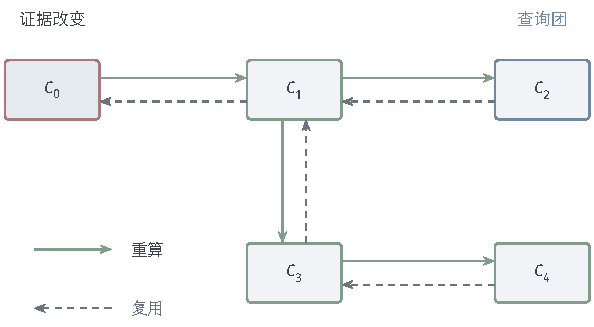
\includegraphics[width=100.651mm]{figures/06-probabilistic-graphical-models/02-inference/tikz/pgm-junction-tree-evidence-update/figure.pdf}
  \caption{单个团势变化后的消息更新。$C_0$改变后，实线方向重新汇总含$C_0$一侧的贡献，反向虚线消息继续复用。查询$C_2$只需更新$C_0-C_1-C_2$路径；其他团表需在其入站消息也更新后才能用于新证据。团的具体变量集合仍须满足运行交集性质。}
  \label{fig:pgm-junction-tree-evidence-update}
\end{figure}

报警例中新观测到$S=0$，变化仅发生在$C_2$。保留$m_{C_1\to C_2}=(0.83,0.17)$，重算$m_{C_2\to C_1}=(0.0095,0.855)$，得到$Z_{\bm e}=p(A=1,S=0)=0.153235$，故障后验为$0.068590/0.153235\approx0.447613$。若将原先单独的报警证据改为$A=0$，反向消息变为$(0.9555,0.0955)$，证据概率为$0.80930$，故障后验为$0.02675/0.80930\approx0.033053$。这两次修改都保留故障侧的先验汇总。

撤回硬证据需要从原始输入恢复团势。旧指示函数已把部分表项置零，对其相除无法找回这些值，因此保留$\phi_C^0$及每条当前证据，按式~\eqref{eq:pgm-junction-tree-local-evidence}重新形成受影响的局部势。随后按源侧依赖重算消息及其缩放常数。若先前还按证据删去变量或裁剪连接，撤回时需一并恢复这些结构。

在原有作用域内修改因子数值，或加入被现有团覆盖的观测似然，都可以沿当前团树更新。新作用域超出现有团时，则要重新分配因子、扩大团或重新三角化，以容纳新增的共同变量。更新后若$Z_{\bm e}=0$，包括硬证据互相矛盾的情形，传播得到零总权重，条件后验没有定义。缓存更新因而同时依赖作用域覆盖、消息来源和正的归一化常数。

\section{算法分析}
\label{sec:pgm-junction-tree-analysis}

\subsection{正确性与校准}
\label{sec:pgm-junction-tree-correctness}

校准给出重叠表的一致性，消息的子树含义则把这些表与原始模型联系起来。下面将一条消息写成源侧全部局部势的求和，进而证明团表确实是所需边缘；同一含义也确定跨团查询的边界和证据更新的依赖范围。

\begin{theorem}[子树消息与团边缘]
  \label{thm:pgm-junction-tree-correctness}
  设$V$为有限变量索引集，每个$X_i$的状态空间有限非空；$\mathcal{T}=(\mathcal{C},\mathcal{E}_{\mathcal T})$是以$V$的子集为团节点、满足$\bigcup_{C\in\mathcal C}C=V$和运行交集性质的有限树。有限个取有限非负值的因子与证据因子恰好各分配给一个覆盖其作用域的团，所得团势为$\phi_C$，并记未归一化目标$q_{\bm e}(\bm{x})=\prod_{C\in\mathcal C}\phi_C(\bm{x}_C)$。对边$(C,D)$，令$S_{C,D}=C\cap D$；删除该边后，记$C$侧的团集合为$\mathcal{C}_{C\mid D}$，并令$U_{C\mid D}=\bigcup_{K\in\mathcal{C}_{C\mid D}}K$。若按式~\eqref{eq:pgm-junction-tree-clique-message}完成全部未缩放和积消息，则对每条有向边$C\to D$，
  \begin{equation}
    m_{C\to D}(\bm{x}_{S_{C,D}})
      =\sum_{\bm{x}_{U_{C\mid D}\setminus S_{C,D}}}
         \prod_{K\in\mathcal{C}_{C\mid D}}\phi_K(\bm{x}_K).
    \label{eq:pgm-junction-tree-subtree-invariant}
  \end{equation}
  完整传播后，定义
  \[
    \begin{aligned}
      B_C(\bm{x}_C)&\mathrel{:=}
        \phi_C(\bm{x}_C)
        \prod_{K\in N_{\mathcal{T}}(C)}
          m_{K\to C}(\bm{x}_{S_{K,C}}),\\
      B_{C,D}(\bm{x}_{S_{C,D}})&\mathrel{:=}
        m_{C\to D}(\bm{x}_{S_{C,D}})
        m_{D\to C}(\bm{x}_{S_{C,D}}),\\
      Z_{\bm e}&\mathrel{:=}
        \sum_{\bm{x}_V}q_{\bm e}(\bm{x}).
    \end{aligned}
  \]
  则对任意团$C$及边$(C,D)$，
  \begin{equation}
    \begin{aligned}
      B_C(\bm{x}_C)
        &=\sum_{\bm{x}_{V\setminus C}}q_{\bm{e}}(\bm{x}),\\
      B_{C,D}(\bm{x}_{S_{C,D}})
        &=\sum_{\bm{x}_{V\setminus S_{C,D}}}q_{\bm{e}}(\bm{x}).
    \end{aligned}
    \label{eq:pgm-junction-tree-true-marginals}
  \end{equation}
  若$Z_{\bm e}>0$，则$B_C/Z_{\bm e}$与$B_{C,D}/Z_{\bm e}$分别为相应的后验团边缘和后验分隔集边缘。
\end{theorem}

\begin{proof}
  按源侧$\mathcal C_{C\mid D}$的团数归纳。若只有叶团$C$，这一侧的全部输入就是$\phi_C$，消去$C\setminus S_{C,D}$即得到式~\eqref{eq:pgm-junction-tree-subtree-invariant}。

  对源侧含多个团的情况，删除$C$后，除$D$侧外的每个邻团$K$各形成一个分支，内部变量为$R_K=U_{K\mid C}\setminus S_{K,C}$。若变量同时出现在该分支和$C$，连接两处的路径经过$K$，运行交集使它属于$S_{K,C}$，所以$R_K$与$C$不交。若两个分支的内部集合共享某变量，连接这两处的路径经过$C$，运行交集又要求它属于$C$，与内部变量定义矛盾。因此各$R_K$彼此也不交。

  要消去的$U_{C\mid D}\setminus S_{C,D}$由$C\setminus S_{C,D}$和各分支内部$R_K$组成。固定$\bm{x}_C$后，这些分支可以分别求和，归纳假设将每一项识别为$m_{K\to C}$。再用有限求和的分配律，可得
  \[
    \begin{aligned}
      &\sum_{\bm{x}_{U_{C\mid D}\setminus S_{C,D}}}
         \prod_{L\in\mathcal{C}_{C\mid D}}\phi_L\\
      &\quad=\sum_{\bm{x}_{C\setminus S_{C,D}}}\phi_C
         \prod_{K\in N_{\mathcal{T}}(C)\setminus\{D\}}
          \left[
            \sum_{\bm{x}_{R_K}}
              \prod_{L\in\mathcal{C}_{K\mid C}}\phi_L
          \right]\\
      &\quad=\sum_{\bm{x}_{C\setminus S_{C,D}}}\phi_C
         \prod_{K\in N_{\mathcal{T}}(C)\setminus\{D\}}m_{K\to C}.
    \end{aligned}
  \]
  该式最后一行就是$C\to D$的更新公式，因此归纳式对整个源侧成立。

  固定任意团$C$，用同样的分解纳入全部邻接分支。它们的内部变量互不重叠，与$C$共同覆盖$V$，局部势又各出现一次，乘积为$q_{\bm e}$。先对各分支内部求和，就留下$\phi_C\prod_Km_{K\to C}=B_C$，得到团边缘等式。再对$C\setminus S_{C,D}$求和，式~\eqref{eq:pgm-junction-tree-local-calibration}给出分隔集边缘$B_{C,D}$。将任一表对其全部状态求和，均得$Z_{\bm e}$；若它为正，归一化即得后验边缘。
\end{proof}

这项证明逐一使用了两个结构条件：运行交集把全部共享变量留在分隔集中，使各分支的内部变量互不重叠；唯一因子分配使局部势的乘积恰为输入模型。于是分配律可以把全局求和拆成消息。仅从一组归一化且相邻一致的表出发，可以重构满足它们的分布，但要确认它就是原模型，还需要上述与原始因子乘积的联系。

在相同的子树分解中，将求和换成最大化，非负因子的分配律给出最大积消息的最优值。给定分隔集状态，回溯表保存的内部选择取得这条消息的值；每次展开时，已有赋值与新分支仅在分隔集中重叠。沿树代入这些选择，最终配置的联合权重就达到根的最大值。根最大值为零时，全部配置的权重都为零，条件分布及其条件MPE均没有定义。

因子和消息可以含零表项，和积与最大积证明都仍成立；正表项主要便于采用比值形式重构。连续变量的和积消息改用积分，需要合适的密度、有限且为正的归一化常数，以及能够精确计算的局部积分。Tonelli定理允许交换非负函数的积分次序，实际积分表达仍取决于函数形式。连续观测还需要相应的条件密度或观测模型，单点指示函数在通常连续测度下无法直接产生离散硬证据那样的概率质量。

\subsection{与变量消除的关系}
\label{sec:pgm-junction-tree-ve-relation}

三角化记录了变量消除产生的共同作用域。消去$v_i$时，相关因子的乘积作用域包含在$\{v_i\}\cup N_i^+$中，输出以剩余邻居$N_i^+$为边界。保存每个消元集合及其生成的新因子，就可以记录这些局部计算之间的消息依赖。最大权团树选择进一步为极大团之间确定满足运行交集的连接（参见\BookTheoremRef{thm:graph-theory-clique-tree-maximum-weight}{卷1《数学准备：计算、分析与几何》第9章“图的表示与计算”第9.3.2.3节“弦图条件下的无填充分解”}）。

收缩被相邻较大集合包含的非极大集合，相当于将数步局部消元合并为一次团间计算，得到更紧凑的团树。此时一条极大团间消息可以汇总连续消去的多个变量，消息与单个消元步骤之间未必一一对应。

从团树也可以恢复消元过程。选定根后，在叶团中消去不属于父分隔集的变量；运行交集保证这些变量已不在其他未处理团中出现。把生成的分隔集因子送入父团，继续处理，便完成收集阶段。因此两种算法使用同样的乘法和边缘化，并由同样的子问题分解保证精确性。

以报警例的$C_1=\{F,H\}$为根时，先在$C_2$内用报警指示函数固定$A$，再对$A,S$求和形成$u(h)$；根结合自身势，再消去$H$得到故障查询。以$C_2$为根时，$C_1$消去$F$形成$v(h)$。保存这两个方向的表，后续就能读取$F,H,S$的边缘，避免重新进行故障侧或报警侧的消元。

查询次数决定了保存消息的收益。只求一次目标边缘时，变量消除可以及时释放已经用完的中间表，收集到目标位置即可。固定模型上反复读取不同位置的边缘，或多次局部修改证据时，团树的双向消息提供持续复用。缓存同样可以用于变量消除；团树将它组织成明确的源侧依赖和失效规则\scite{pgm-koller2009}

\subsection{复杂度与适用边界}
\label{sec:pgm-junction-tree-complexity}

一轮传播只发送与树边数成正比的消息，每张消息的计算量还取决于团的状态空间。令$k=|\mathcal C|$、$r_i=|\mathcal X_i|$，团表和分隔集表分别有
\begin{equation}
  r_C=\prod_{i\in C}r_i,\qquad
  r_{C,D}=\prod_{i\in S_{C,D}}r_i.
  \label{eq:pgm-junction-tree-table-sizes}
\end{equation}
发送$C\to D$输出$r_{C,D}$个数。通用稠密实现通常先遍历$r_C$个团状态，组合势和各入站消息，再累加到对应的分隔集状态。因此，即使分隔集表很小，形成它仍可能需要枚举一个大团。

若团$C$的度为$\deg(C)$，逐条出站消息都重乘其余入站消息，会重复执行$O(\deg(C)^2r_C)$次乘法。可以对每个团状态计算入站值的前缀积和后缀积，以$O(\deg(C))$次乘法得到排除任意邻居的乘积，再分别累加。这种做法保留零表项，避免除以某个零消息。配合收集和分发，完整传播的时间上界为
\begin{equation}
  O\!\left(\sum_{C\in\mathcal{C}}(\deg(C)+1)r_C\right),
  \label{eq:pgm-junction-tree-time}
\end{equation}
这个上界从已建好的局部势开始计算，并假定表索引等基本操作成本有界；$+1$计入形成团汇总表的遍历。如果每条消息各自重新组合全部输入，则还需计入重复乘法产生的度数因子。

局部势、团汇总表以及边的两个方向消息需要持久保存，内存规模为
\begin{equation}
  O\!\left(
    \sum_{C\in\mathcal{C}}r_C+
    2\sum_{(C,D)\in\mathcal{E}_{\mathcal{T}}}r_{C,D}
  \right),
  \label{eq:pgm-junction-tree-memory}
\end{equation}
输入因子、工作空间和最大积回溯表需另外计入。前缀积与后缀积可逐个团状态临时计算，使用后释放。只保存消息、查询时再重建团表，也可减少持久存储的常数开销；每张实际需要的稠密团表仍取决于团状态数。

若单变量状态数至多为$r$，所选三角化的最大团大小为$w+1$，则$r_C\le r^{w+1}$。树上$\sum_C\deg(C)=2(k-1)$，代入式~\eqref{eq:pgm-junction-tree-time}得到$O(kr^{w+1})$；对$m$个原始因子，按稠密表建立局部势的保守成本为$O(mr^{w+1})$。不同极大团的分隔集至多含$w$个变量，因此消息表至多有$r^w$项，团势表则至多有$r^{w+1}$项。这里$w$属于已选顺序，最优三角化才使它等于原交互图的树宽。

变量状态数不同时，同样大小的团也可能需要不同规模的表。对图~\ref{fig:pgm-junction-tree-triangulation}中的四环，取$r_1=r_3=10$、$r_2=r_4=2$，表~\ref{tab:pgm-junction-tree-triangulation-cost}展示两种填充选择。两个方案都产生三变量团，但团表和分隔集表项数显著不同，因此排序时还需考虑各变量状态数。

\begin{table}[htbp]
  \centering
  \begin{tabular}{cccc}
    \toprule
    填充边 & 极大团 & 各团表项数 & 分隔集表项数\\
    \midrule
    $1-3$ & $\{1,2,3\},\{1,3,4\}$ & $200,\;200$ & $100$\\
    $2-4$ & $\{1,2,4\},\{2,3,4\}$ & $40,\;40$ & $4$\\
    \bottomrule
  \end{tabular}
  \caption{四环的两种三角化及其表规模。人工设置$r_1=r_3=10$、$r_2=r_4=2$，两种方案的未加权树宽同为$2$，但填充边$2-4$对应的团表与消息表更小。}
  \label{tab:pgm-junction-tree-triangulation-cost}
\end{table}

大团很快会占满内存：$30$个二元变量组成的团有$2^{30}$个表项，一张双精度表就占$8$\,GiB，还需保存其他团、消息和工作空间。最大权选树发生在极大团形成之后，无法缩小这些表。单团证据变化最坏仍需向全树传播；跨团联合查询还要进行子树内消元，并写出可能很大的查询表。

上述指数界针对稠密离散表表示。满足积分条件的高斯势使用精度矩阵和一次项，消息通过块矩阵消元形成，成本取决于矩阵维数和填充。紧凑表示依赖函数族在乘法与积分下保持闭包；混合分量增加或一般非线性势可能使消息变得更复杂。因此评估成本时，应把实际的局部积分、最大化或枚举方式一并计入。

团树适用于作用域固定、可摊销编译成本且团表可容纳的重复推断。稠密团表的规模过大时，需要改用更紧凑的函数表示或近似推断。第~\ref{sec:pgm-variational-bethe}节会讨论直接在含环图上迭代消息的方法；那时分支可能重叠，须另行分析固定点和近似误差。

\section{本章小结}
\label{sec:pgm-junction-tree-summary}

消息将一侧子问题的内部变量汇总掉，保留后续计算所需的边界状态。因子树可以直接按边切分，一般图则先以道德化和三角化确定共同作用域，再将团连成运行交集树。共享变量沿路径连续保留，原始因子各分配一次，这两项条件使消息能够精确组合为原模型的边缘。

收集汇总根的各侧贡献，分发为其他团补齐根侧信息。若$Z_{\bm e}>0$，$B_C/Z_{\bm e}$给出团的后验边缘，$\phi_C$继续保存本团的原始输入。单团覆盖的查询在团内求和；跨团查询借助边界消息继续消元，或用分隔集势修正重叠权重。MPE另用最大积消息和回溯表恢复最优配置。证据改变时，按源侧依赖更新缓存；撤回硬证据则从原始团势恢复输入。

团树保存的不仅是数值结果，还有每张表与局部因子的依赖关系，使多次查询和局部更新可以共享已经完成的计算。最大团的状态空间、各变量状态数和查询输出大小仍决定存储与算术成本，缓存主要节省重复消元的工作。

\paragraph{扩展阅读}
Lauritzen与Spiegelhalter的局部计算论文介绍如何通过图变换组织概率计算，Koller与Friedman的教材系统推导团树传播。两者可结合本章的子树不变量阅读：运行交集确定完整边界，证据分配确定输入乘积，校准则给出共享变量上一致的边缘\scite{pgm-overview-lauritzen1988,pgm-koller2009}
